\documentclass{article}

\usepackage[a4paper]{geometry}
\usepackage{pablo}


\begin{document}

\thispagestyle{empty}

\begin{center}
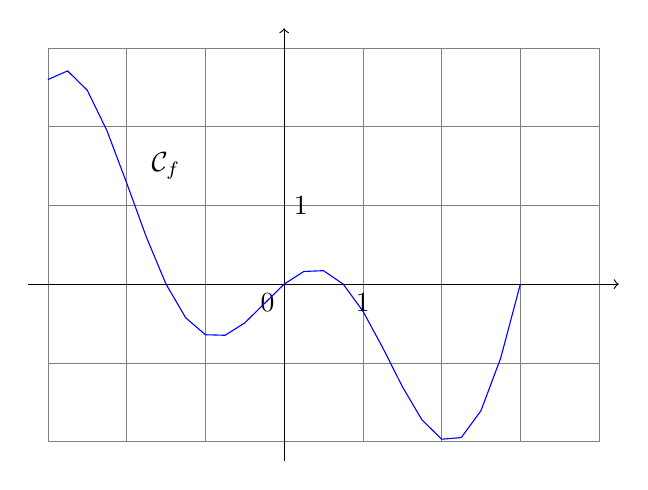
\begin{tikzpicture}[domain=-3:4, scale=1]
\draw[very thin,color=gray,step=1] (-3,-2) grid (4,3);
\draw[->] (-3.25,0) -- (4.25,0);
\draw (1,0) node[below] {1};
\draw[->] (0,-2.25) -- (0,3.25);
\draw (0,1) node[right] {1};
\draw (0,0) node[below left] {0};
\draw[color=blue,domain=-3:3]
plot (\x,{\x * cos(80*\x + 30)});
\draw (-1.5,1.5) node {${\cal C}_f$};
\end{tikzpicture}
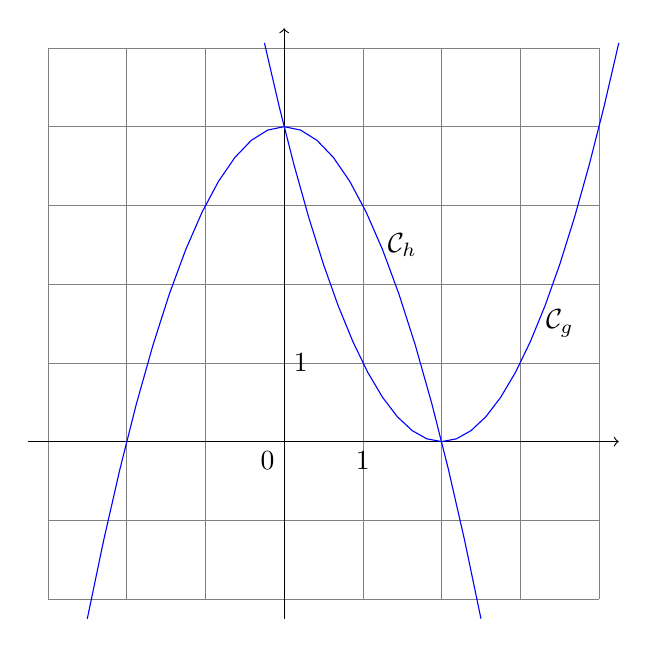
\begin{tikzpicture}[domain=-3:4, scale=1]
\draw[very thin,color=gray,step=1] (-3,-2) grid (4,5);
\draw[->] (-3.25,0) -- (4.25,0);
\draw (1,0) node[below] {1};
\draw[->] (0,-2.25) -- (0,5.25);
\draw (0,1) node[right] {1};
\draw (0,0) node[below left] {0};
\draw[color=blue,domain=-2.5:2.5]
plot (\x,{-(\x-2)*(\x+2)});
\draw (3.5,1.5) node {${\cal C}_g$};
\draw[color=blue,domain=-0.25:4.25]
plot (\x,{(\x-2)*(\x-2)});
\draw (1.5,2.5) node {${\cal C}_h$};
\end{tikzpicture}
\end{center}

\vspace{\stretch{1}}

\begin{center}
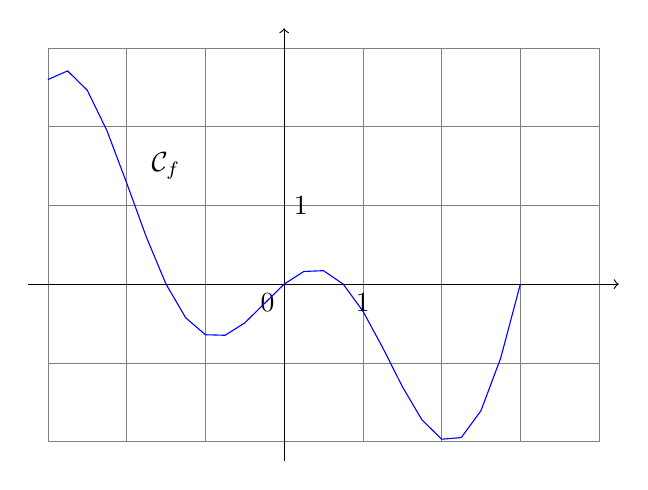
\begin{tikzpicture}[domain=-3:4, scale=1]
\draw[very thin,color=gray,step=1] (-3,-2) grid (4,3);
\draw[->] (-3.25,0) -- (4.25,0);
\draw (1,0) node[below] {1};
\draw[->] (0,-2.25) -- (0,3.25);
\draw (0,1) node[right] {1};
\draw (0,0) node[below left] {0};
\draw[color=blue,domain=-3:3]
plot (\x,{\x * cos(80*\x + 30)});
\draw (-1.5,1.5) node {${\cal C}_f$};
\end{tikzpicture}
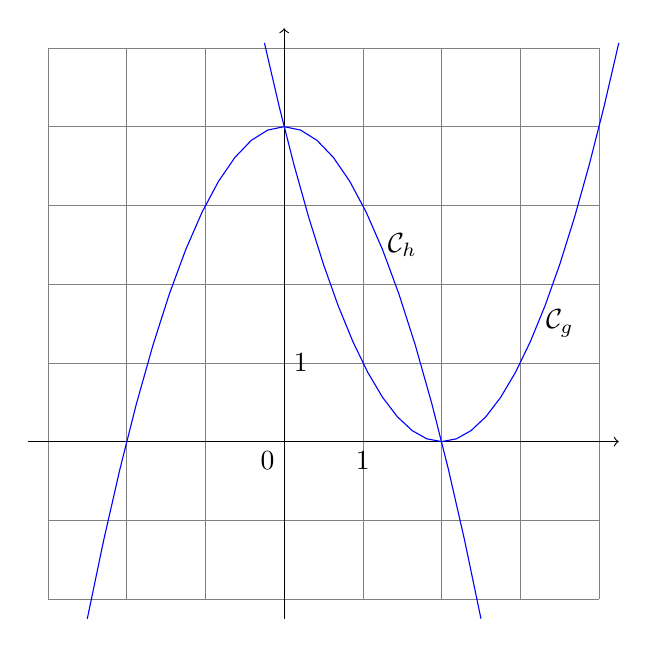
\begin{tikzpicture}[domain=-3:4, scale=1]
\draw[very thin,color=gray,step=1] (-3,-2) grid (4,5);
\draw[->] (-3.25,0) -- (4.25,0);
\draw (1,0) node[below] {1};
\draw[->] (0,-2.25) -- (0,5.25);
\draw (0,1) node[right] {1};
\draw (0,0) node[below left] {0};
\draw[color=blue,domain=-2.5:2.5]
plot (\x,{-(\x-2)*(\x+2)});
\draw (3.5,1.5) node {${\cal C}_g$};
\draw[color=blue,domain=-0.25:4.25]
plot (\x,{(\x-2)*(\x-2)});
\draw (1.5,2.5) node {${\cal C}_h$};
\end{tikzpicture}
\end{center}

\vspace{\stretch{1}}

\begin{center}
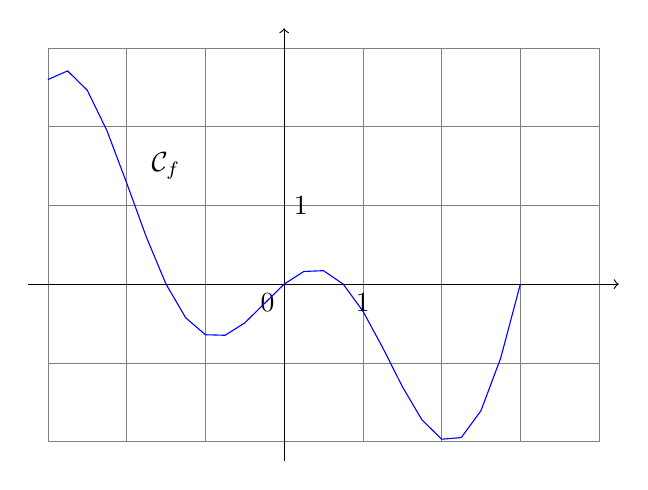
\begin{tikzpicture}[domain=-3:4, scale=1]
\draw[very thin,color=gray,step=1] (-3,-2) grid (4,3);
\draw[->] (-3.25,0) -- (4.25,0);
\draw (1,0) node[below] {1};
\draw[->] (0,-2.25) -- (0,3.25);
\draw (0,1) node[right] {1};
\draw (0,0) node[below left] {0};
\draw[color=blue,domain=-3:3]
plot (\x,{\x * cos(80*\x + 30)});
\draw (-1.5,1.5) node {${\cal C}_f$};
\end{tikzpicture}
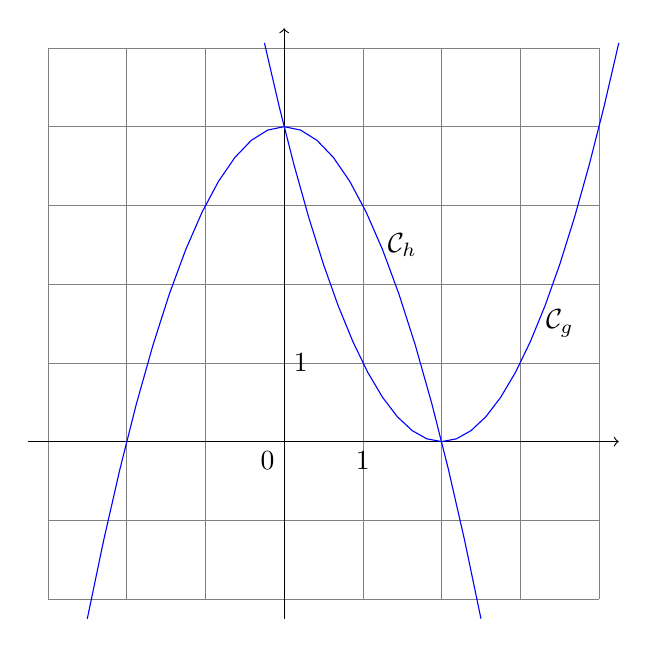
\begin{tikzpicture}[domain=-3:4, scale=1]
\draw[very thin,color=gray,step=1] (-3,-2) grid (4,5);
\draw[->] (-3.25,0) -- (4.25,0);
\draw (1,0) node[below] {1};
\draw[->] (0,-2.25) -- (0,5.25);
\draw (0,1) node[right] {1};
\draw (0,0) node[below left] {0};
\draw[color=blue,domain=-2.5:2.5]
plot (\x,{-(\x-2)*(\x+2)});
\draw (3.5,1.5) node {${\cal C}_g$};
\draw[color=blue,domain=-0.25:4.25]
plot (\x,{(\x-2)*(\x-2)});
\draw (1.5,2.5) node {${\cal C}_h$};
\end{tikzpicture}
\end{center}

\end{document}
